\documentclass[]{interact}

\usepackage{epstopdf}% To incorporate .eps illustrations using PDFLaTeX, etc.
\usepackage[caption=false]{subfig}% Support for small, `sub' figures and tables
%\usepackage[nolists,tablesfirst]{endfloat}% To `separate' figures and tables from text if required
%\usepackage[doublespacing]{setspace}% To produce a `double spaced' document if required
%\setlength\parindent{24pt}% To increase paragraph indentation when line spacing is doubled
\usepackage{svg}
%\usepackage{biblatex}
\usepackage[numbers,sort&compress]{natbib}% Citation support using natbib.sty
\bibpunct[, ]{[}{]}{,}{n}{,}{,}% Citation support using natbib.sty
\renewcommand\bibfont{\fontsize{10}{12}\selectfont}% Bibliography support using natbib.sty
\makeatletter% @ becomes a letter
\def\NAT@def@citea{\def\@citea{\NAT@separator}}% Suppress spaces between citations using natbib.sty
\makeatother% @ becomes a symbol again

\theoremstyle{plain}% Theorem-like structures provided by amsthm.sty
\newtheorem{theorem}{Theorem}[section]
\newtheorem{lemma}[theorem]{Lemma}
\newtheorem{corollary}[theorem]{Corollary}
\newtheorem{proposition}[theorem]{Proposition}

\theoremstyle{definition}
\newtheorem{definition}[theorem]{Definition}
\newtheorem{example}[theorem]{Example}

\theoremstyle{remark}
\newtheorem{remark}{Remark}
\newtheorem{notation}{Notation}

\begin{document}

%\articletype{ARTICLE TEMPLATE} Specify the article type or omit as appropriate

\title{Behavioural Analysis of Independent Value-Based Learning in Non-cooperative Games}

\author{
\name{Yang Li\textsuperscript{a}\thanks{CONTACT Yang Li. Email: yang4.li@uwe.ac.uk}, Marco Perez Hernandez\textsuperscript{a} and Mehmet Emin Aydin\textsuperscript{a}}
\affil{\textsuperscript{a} University of the West of England, Frenchay Campus, Coldharbour Lane, Bristol, UK}
}

\maketitle

\begin{abstract}
Multi-agent reinforcement learning has received increased attention in cooperative games. However, research in non-cooperative games is lagging behind. Independent value-based learning algorithms have demonstrated simplicity and versatility in various contexts. In this paper, we study the behaviour of these algorithms in non-cooperative settings. We explain the conditions that a game must satisfy for the algorithms to work. We further test the algorithms in our proposed game Food Chain that simulates an ecosystem. Our results show that independent value-based learning algorithms can converge to Nash equilibrium, only when the Nash equilibrium consists of uniformly random policies over the feasible actions.
\end{abstract}

\begin{keywords}
Multi-agent reinforcement learning; independent value-based learning; game theory; non-cooperative games; Nash equilibrium
\end{keywords}

\section{Introduction}
Recent multi-agent reinforcement learning (MARL) research has mostly focused on fully cooperative games \cite{yu2020benchmarking, papoudakis2020benchmarking, zhu2024survey} where there is no conflict between agents as they share a common reward. When agents are allowed to share information, we can apply single-agent reinforcement learning (RL) algorithms to a fully cooperative game where the collective agent tries to find the optimal joint action, given the joint observation, although the problem is still challenging in practice because of what the computational complexity of the joint action brings. In a traditional single-agent setting, the agent needs to learn which action gives the best reward. A Pareto-optimal pure strategy is guaranteed to exist in fully cooperative finite games, meaning that the agents can always deterministically choose the optimal action that has the highest payoff.

Non-cooperative environments, however, involve conflicts that make learning more complicated. Agents may belong to different parties that would like to have private control to protect their own interests. Rational and self-interested agents will have to fight for what is best for them, as increasing one agent's reward might lead to the decline of other's gains. We can no longer intuitively define the solution for a game as the optimal strategy resulting in the highest reward. One of the possible solution concepts is the Nash equilibrium (NE). NEs describe the stable points in games, which are associated with the convergence to optimal behaviour of agents.

Many real-world problems can be modelled as non-cooperative games, such as business competition, political campaigns, stock trading, bidding in auctions, cyber security, and traffic routing. For example, if we omit the long-term economic growth, the stock market is often considered a 0-sum fully competitive game where one person's profit is another person's loss. Another example is cyber security, which must study the conflicts between attackers and defenders. These problems feature the competitive nature of games because they share one thing in common, parties with conflicting interests. Substantial research has been done on MARL in fully cooperative games, and non-cooperative games have received less attention \cite{zhu2024survey, li2024fightladder}.

Some studies have explored the application of MARL to solve games. One of which is independent value-based learning (IVBL). IVBL is a family of algorithms that models the multi-agent environments as single-agent environments, and they compute for each agent the expected reward of each action under each state. IVBL is simple and highly scalable because it is decentralized. It has been adopted for both cooperative \cite{foerster2017stabilising, omidshafiei2017deep, palmer2017lenient, palmer2018negative} and non-cooperative tasks \cite{bjornsson2009cadiaplayer, jiang2018q, qu2020distributed, kopacz2023evaluating}. This paper analyses the performance of IVBL in non-cooperative finite games. The analysis considers characteristics of the action space and the NEs of the game, combining both formal analysis and experimental evaluation in selected two-player non-cooperative games. The results show NEs with uniformly random policies is a necessary condition for stability convergence of IVBL algorithms in non-cooperative environments. These condition highly restricts the wider applicability of IVBL.

%\subsection{Main contributions}
The main contributions of this work include the following points:
\begin{itemize}
    \item Behavioural analysis identifying necessary conditions for a stable convergence of IVBL which can drive the choice of algorithms in non-cooperative finite games.
    \item Introducing a non-cooperative game that has the characteristics which challenge the agents from a game theory perspective aligned with our analysis.
    \item Experimental evaluation of IVBL algorithms in selected two-player scenarios in the game proposed above.
\end{itemize}

%\subsection{Contents}
The remainder of the paper is organized as follows:
The next section provides the literature review on the key features of non-cooperative games and the most popular MARL algorithms that is related to our work. We then state the formal definitions of games and other concepts discussed in this paper in Section 3. Section 4 analyses the stability of IVBL in non-cooperative games. To verify our analysis with experimental results, a new game called Food Chain is introduced in Section 5. The game will have the key features discussed in our analysis that bring specific challenges to MARL agents. Then, we present the design as well as the results of our experiments and relevant discussions in Section 6. Finally, the drawn conclusions pulled in the last section.

\section{Background and Literature Review}
This literature review focuses on key features of non-cooperative games, as well as the MARL approaches to solve these games.

\subsection{Non-Cooperative Games}
In single-agent or fully cooperative environments, there is one reward function for all agents. Thus, the agents only need to learn which (joint) action has the highest payoff. In non-cooperative games, there may be no optimal joint action that satisfy all agents. Several problem solving concepts/approaches for non-cooperative games are discussed in game theory \cite{albrecht2024multi}. These include Pareto optimum, Nash equilibrium, and correlated equilibrium. Nash Equilibrium (NE), proposed by John Nash, is a renown approach for non-cooperative games \cite{nash2024non}. NE offers a framework to characterise and analyse stability in games and describes a stability condition with which no player can benefit from deviating from their current strategy independently. The stability is associated to the optimal outcome in non-cooperative games and hence the objective agents aim for. Generally, there may only be a mixed NE, meaning that players must adopt randomized action-selection policy consisting of probability distributions over the action space. This is the mixed policy problem.

Many fully competitive games are studied in the MARL community such as Pommerman \cite{resnick2018pommerman}, Go \cite{silver2017mastering}, StarCraft II \cite{vinyals2019grandmaster}, and Dota 2 \cite{berner2019dota}. There are also some general non-cooperative environments such as hide-and-seek \cite{baker2019emergent}, Neural MMO \cite{suarez2021neural}. PettingZoo and Melting Pot \cite{terry2021pettingzoo, leibo2021scalable} are two integrated MARL environments including many cooperative and non-cooperative games. Kopazs et al. \cite{kopacz2023evaluating} studied the non-cooperative game predator-and-prey in the PettingZoo library, which is closely related to the game defined in this work. However, we lack a standard benchmark for MARL algorithms in non-cooperative games due to the difficulty of measuring agents' performance in general non-cooperative games. In cooperative games, the reward simply increases as the agents do better at the game. However, this is not the case in non-cooperative games where increasing one agent's outcome often results in the drop of another agent's return. FightLadder \cite{li2024fightladder} used the Elo rating system to test MARL algorithms but they were restricted to two-player zero-sum fighting games.

\subsection{MARL Algorithms}
Independent learning (IL) algorithms that are carried over from the traditional single-agent RL domain treat other agents as part of the environment. The agents are essentially unaware of the existence of one another. IL algorithms are popular for handling many complex problems \cite{papoudakis2020benchmarking, gupta2017cooperative, de2020independent, palmer2020independent}. Among these, independent value-based learning (IVBL) algorithms, such as the classic independent Q-learning (IQL) \cite{tan1993multi}, learn the expected long-term cumulative return (the Q-value) of each action at each state through sampling. IVBL algorithms including IQL are often considered as baseline and natural choice in a wide range of MARL studies because of their simplicity and scalability. For example, they were studied in various cooperative environments \cite{foerster2017stabilising, omidshafiei2017deep, palmer2017lenient, palmer2018negative}. The problem is that IVBL agents only help produce the average reward of each action for each agent, but do not pay attention on what the action-selection policy. This is not a problem in single-agent or cooperative environments as we can simply pick the action with the highest return. Some studies addressed this issue in non-cooperative games by simply choosing the action with the highest empirical return \cite{bjornsson2009cadiaplayer, jiang2018q, kopacz2023evaluating} and observed reasonably good outcome. Kopacz et al \cite{kopacz2023evaluating} has examined IVBL in the non-cooperative game predator-and-prey. Both the algorithm and the game are closely related to our work. Other researchers \cite{qu2020distributed} tried to address this problem using the softmax function given in Equation~(\ref{eq:softmax}) to calculate a policy based on the payoff. Softmax takes a vector as input and computes a probability distribution over the original vector entries, such that the higher the original value, the higher the probability.
\begin{equation}
    \textbf{softmax}([x_1, ..., x_n]) = [\frac{e^{x_1}}{\sum_{i}{e^{x_i}}}, ..., \frac{e^{x_n}}{\sum_{i}{e^{x_i}}}]
    \label{eq:softmax}
\end{equation}
The latter approach emphasis the action with higher empirical return. However, these approaches have a problem that guarantees failure of learning in a wide range of games. We will take a closer look in the analysis section.

Unlike IL, joint action learning (JAL) algorithms allow the agent to gain access to the information processed by all other agents, such as their choices of actions, so agents can learn the expected return of joint actions. Minimax Q-learning \cite{littman1994markov} is a JAL algorithm that can be applied to two-player zero-sum games. It computes local minimax solutions for each state based on the learned joint Q-values. Nash Q-learning \cite{hu2003nash} is a similar algorithm that computes the local NE instead. It converges to a NE under highly strict assumptions that reduce the applicability of the approach to a limited set of games. Correlated Q-learning \cite{greenwald2003correlated} computes a correlated equilibrium and has no known convergence guarantees. Zinkevich et al \cite{zinkevich2005cyclic} showed that JAL cannot converge in certain types of ill-conditioned games. Centralized learning requires full knowledge of the action spaces of all agents, which may not always be available if we are dealing with real-world problems. Another major disadvantage is that the number of joint actions is the number of possible combinations of the individual actions. This introduces combinatorics to the computational complexity of our algorithms, making them unscalable.

In contrast to the value-based approach, policy-based algorithms, such as the policy gradient methods, work around this issue by learning the policies directly, without putting an estimation on the individual action return. Policy gradient methods optimize a parametrized policy function using gradient decent to maximize the return. An advantage of policy gradient methods is that they naturally work on continuous action spaces. The actor-critic algorithms are a family of RL algorithm which trains a parametrized policy called the actor and a state-value function called the critic to estimate the policy gradient. Soft actor-critic (SAC) \cite{haarnoja2018soft} has become one of the most popular algorithms recently. Its multi-agent variant (MASAC) has been considered the state-of-the-art (SOTA) baseline \cite{yu2020benchmarking, zhang2020lyapunov}. There is also naturally an independent version (ISAC) for MARL. The proximal policy optimization algorithm (PPO) \cite{schulman2017proximal} was based on actor-critic as well and was extended to multi-agent environments by some researchers \cite{yu2020benchmarking, yu2022surprising} (MAPPO). Surprisingly, the IL version of PPO (IPPO) has proven to substantially outperform MAPPO and other algorithms in some cooperative tasks in StarCraft II \cite{de2020independent}. MADDPG \cite{lowe2017multi} is another policy gradient algorithm that is often considered SOTA. Because it only works for continuous action spaces, we do not discuss them further in the context of finite games.

Other notable MARL algorithms that have shown good performance include VDN \cite{sunehag2017value} and its improved version QMIX \cite{rashid2020monotonic}. The weakness is that they can only work for fully cooperative games where agents share a common reward.

\subsection{Summary}
As shown in this review, the issue of deriving the policy from the Q-values learned by IVBL agents in non-cooperative games has not been fully addressed by the MARL community, \cite{bjornsson2009cadiaplayer, jiang2018q, kopacz2023evaluating, qu2020distributed} made progress in this direction, but they did not analyse the behaviour of the agents and identify the flaws from a game theory point of view.

\section{MARL Preliminaries}
In this section, we provide preliminaries including the formal definition of a game and NE.

\subsection{Stochastic Game}
A game is formally defined by a tuple:

$G = \langle N,S,S_0,S_t,\{A_1,\ldots,A_n\},\{R_1,\ldots,R_n\},T \rangle$
\begin{itemize}
    \item $N = \{1, ..., n\}$: the set of agents, numbered from 1 to $n$.
    \item $S$: the game’s state space.
    \item $S_0 \subset S$: the set of possible initial states.
    \item $S_t \subset S$: the set of terminal states.
    \item $\{A_1,\ldots,A_n\}$: one action space for each agent. Let $a_i \in A_i$ be an action of agent $i$, and $a^n=\langle a_1,\ldots,a_n \rangle \in A^n$ denote a joint action in the joint action space.
    \item $\{R_1,\ldots,R_n\}$: one reward function for each agent. $R_i:S \times A^n \times S \rightarrow \mathbb{R}$.
    \item $T$: the state transition function. $T:S \times A^n \times S \rightarrow [0,1]$. It defines the probability of the game transitions from one state to another given the joint action. It must satisfy the axiom of probability:
    \begin{equation}
        \forall s \in S,a^n \in A^n: \sum_{s' \in S}{T(s,a^n,s')}=1
        \label{eq:state_transition}
    \end{equation}
\end{itemize}
Starting from a randomly chosen $s_0 \in S_0$, at each time step $t \in \mathbb{N}$ with the current state $s_t$, each agent observes the current state $s_t$ and chooses an action forming a joint action $a^n=\langle a_1,\ldots,a_n \rangle$. The game then moves into the next state $s_{t+1}$, randomly sampled from the distribution P and a reward $R_i$ is assigned to each agent. If $s_t \in S_t$, the game ends. Otherwise, the game continues in the next time step.

The way a player plays the game defines a policy (strategy) as a function that computes the probability of selecting each action given the current state, $\pi:S \times A^n \rightarrow [0,1]$. A strategy is said to be pure if it is deterministic ($\pi:S \times A^n \rightarrow \{0,1\}$). Otherwise, we call it a mixed strategy. A set of strategies, one for each player, is called a profile $\pi^n$. Given the profile, we can compute the expected reward for each player in the game. The goal is to find the optimal strategy for an agent, or even the optimal profile, such that expected cumulative rewards are maximized. Cooperative games are special cases where agents share the same reward. The optimal profile is the one that maximizes the common reward. Because they share the same reward function, the problem can be formulated as a joint player selecting a joint action and receives a reward, which makes cooperative games essentially single-agent games from a game theory perspective. In general non-cooperative games, however, it may not be possible to make everyone happy due to the conflicting interests. A more profound definition of optimum need to be discussed in the non-cooperative games section.

Formally, let $R_i^*(\pi^n)$ be the function to compute the expected reward of the $i^{th}$ player given the profile. Let $\pi_i$ be a policy of the $i^{th}$ player and $\Pi_i$ be the policy space of the $i^{th}$ player. Let $\pi^{-i}$ denote $\pi^n - \{\pi_i\}$, the set of strategies of all other players. A profile $\pi^n$ is a NE if
\begin{equation}
    \forall i \in N, \forall \pi_i \in \Pi_i: R_i^*(\{\pi_i\} \cup \pi^{-i}) \leqslant R_i^*(\pi^n)
    \label{eq:nash}
\end{equation}
The idea is that NEs are the stable points in the game, because if an agent can benefit from switching strategy on its own, they would do so.

A game is finite if $|N|, |S|$ and all $|A_i|$ are finite, and the game always ends in a finite number of turns. John Nash proved that every finite game has at least one NE. To solve a game in the context of this paper means to find at least one NE. Games that are not finite can be ill-conditioned and have no NE. For example, a game where the player who names the greatest number wins has no best strategy. For the rest of the paper, we only refer to finite games. A normal form game has only two states, the starting state $S_0$ and the end state $S_1$. The game ends immediately after all agents pick an action. Thus, they can be represented using the reward matrix. In the book on game theory originally published in 1944 \cite{von2007theory}, Von Neumann and Morgenstern showed that finite games can be translated into normal form games. If we encapsulate the following states as a subgame, we end up with a reward matrix for the initial state with the rewards being the expected rewards of the subgames. We focus on normal form games because they are easier to work with for the analysis. Since they only have one state $S_0$ for agents to take actions, we simply write $\pi(a)$ instead of $\pi(S_0, a)$ to denote the probability of taking action $a$.

\section{Stability of IVBL in Non-Cooperative Games}
In this part of the paper, we show the feasibility of IVBL algorithms in non-cooperative games with behavioural analysis. We demonstrate the necessary conditions the game must satisfy in order to apply the IVBL algorithms.

\begin{table}
    \begin{minipage}{0.5\textwidth}
    \tbl{Rock-Paper-Scissors Reward Matrix}{
    \begin{tabular}{l|ccc}
    & r & p & s\\
    \hline
    r & 0,0 & -1,1 & 1,-1 \\
    p & 1,-1 & 0,0 & -1,1 \\
    s & -1,1 & 1,-1 & 0,0 \\
    \end{tabular}
    }
    \label{table:rps_reward_matrix}
    \end{minipage}
    \begin{minipage}{0.5\textwidth}
    \tbl{Biased Rock-Paper-Scissors Reward Matrix}{
        \begin{tabular}{l|ccc}
        & r & p & s\\
        \hline
        r & 50,50 & 25,75 & 100,0 \\
        p & 75,25 & 50,50 & 45,55 \\
        s & 0,100 & 55,45 & 50,50 \\
        \end{tabular}
    }
    \label{table:biased_rps_reward_matrix}
    \end{minipage}
    \tabnote{The reward matrix is used to define the reward for each player for each choice of action. The row player chooses a row and gets the first reward. Vice versa for the column player.}
\end{table}

To demonstrate the problem with competitive games, we study two simple normal form games. Consider the simple one-shot matrix game rock-paper-scissors (RPS) in Table~\ref{table:rps_reward_matrix}. Each entry represents the reward for the row player and the column player, respectively. The only NE in the game is that two players play each of the three actions with 1/3 chance. If any player deviates from the NE, their expected reward does not increase, and the other player can exploit them by playing the action that counters their most frequent action. Table~\ref{table:biased_rps_reward_matrix} defines a more complicated game called biased rock-paper-scissors. The only NE in the game is that both players adopt the following policy.
\begin{equation}
    \pi=(P(r)=0.0625,P(p)=0.6250,P(s)=0.3125)
    \label{eq:biased_rps_policy}
\end{equation}

A well-known direct consequence of Equation~(\ref{eq:nash}) in game theory is that at any NE $\pi^n$, given the policy set of the other players $\pi^{i-1}$, player $i$ is indifferent from all actions that are chosen with a positive probability \cite{nash2024non}. This means that the actions are split into two sets, the worthy actions that are chosen with a positive probability and the worthless ones that will never be piked. For example, a variation of RPS could incorporate an always-losing action, where the player receives negative reward once executing it, regardless of the opponent’s action. Such an action should never be selected by the players. Additionally, the expected reward will be the same for every worthy action. In other words, the player can choose the worthy actions arbitrarily, given that other players commit to the NE. If we calculate the expected reward of each action in the biased rock-paper-scissors example where the opponent uses the NE strategy, we will see all three actions indeed have the same payoff. The above fact can be formally stated as the following. Assume $\pi^n$ is a NE. Let $Q_i(a_j, \pi^{-i})$ be the expected reward of action $a_j \in A_i$ for agent $i$, given the rest of the profile $\pi^{-i}$. Let $A^+_i$ denote the set of worthy actions of agent $i$, namely $A^+_i = \{a | a \in A_i \wedge \pi_i(a) > 0 \}$. We have:
\begin{equation}
    \begin{aligned}
    \forall a_j, a_k \in A^+_i, Q_i(a_j, \pi^{-i}) = Q_i(a_k, \pi^{-i})
    \label{eq:nash_indifferent}
    \end{aligned}
\end{equation}

Suppose a IVBL algorithm can converge to a NE, then all worthy action's Q-values must converge to the same for an agent. It does not matter how the algorithm computes a probability distribution over the actions at the end, it cannot make any discriminations among those worthy actions based on equal statistics. Such an algorithm will output at best a uniform distribution over the worthy actions at a NE. This contradicts with the assumption that they converge to a NE unless the NE is full of uniformly random policies which is not the case in most of the games. We have shown that pure IVBL approaches does not work through proof by contradiction.

This sets a necessary condition for IVBL algorithms to work. IVBL algorithms can converge to a NE only if the NE consists of uniformly random policies over the set of all worthy actions. Note that this also includes any pure (deterministic) policies. It can be formally stated as follows. Let $\Pi^{n}$ be the set of all possible profiles, and $\Pi^{n*}$ be the subset containing all the NEs.
\begin{equation}
    \exists \pi^n \in \Pi^{n*}, \forall \pi_i \in \pi^n, \forall a_j, a_k \in A^+_i, \pi_i(a_j) = \pi_i(a_k)
    \label{eq:necessary_condition}
\end{equation}
Because in cooperative games, there is no need to use mixed strategies, the NEs are essentially pure. This means that all cooperative games satisfy Equation~(\ref{eq:necessary_condition}), which explains why IVBL works in cooperative games. Additionally, according to Zermelo's theorem \cite{schwalbe2001zermelo}, perfect-information two-player finite asynchronous (players take turns) games such as chess or Go also satisfy the condition, because they also have a pure NE.

Then how did the researchers still find the appealing outcome of IVBL in some non-cooperative games \cite{bjornsson2009cadiaplayer, jiang2018q, kopacz2023evaluating, qu2020distributed}? The behaviour of IVBL can be highly problem-dependent, so we provide only high-level insights here. MARL problems studied in the real world can have large state/action spaces. For example, a $19 \times 19$ Go board can have roughly $3^{19 \times 19} = 10^{172}$ states. It may be too difficult for the agents to converge to a global NE because of the limited computational power. Because of the complexity of the environment mechanics itself, the competitiveness of the game is not going to play an enormous role before agents can reliably predict the state transitions. Picking the action with the best Q-value still gives reasonably good results, since at least the agents learned to interact with the environment.

\section{The Food Chain Game}
To verify our analysis, we test the algorithms in a game that can turn on and off the necessary condition given Equation~(\ref{eq:necessary_condition}) described in the previous section. We define the mechanics of the game Food Chain. An agent in the game represents an animal of some type. They can move around the map and feed themselves while trying to avoid enemies. The game simulates an ecosystem to a certain extend, by defining a food web structure. A food web is a cluster of food chains showing what-eats-what in the ecosystem as illustrated in Figure~\ref{fig:food_chain_game}. The food web in the game is completely customizable and we can define an arbitrary number of species (agent types) and any number of agents of each type. This game is essentially a generalized version of the classic predator-and-prey problem. Recent research has tested IQL in the predator-and-prey game and found the algorithm to be seemingly performing well \cite{kopacz2023evaluating}. As we stated, these results could be misleading.

\begin{figure}
\centering
\subfloat[A Food Web\textsuperscript{1}]{
    \resizebox*{0.48\textwidth}{!}{
        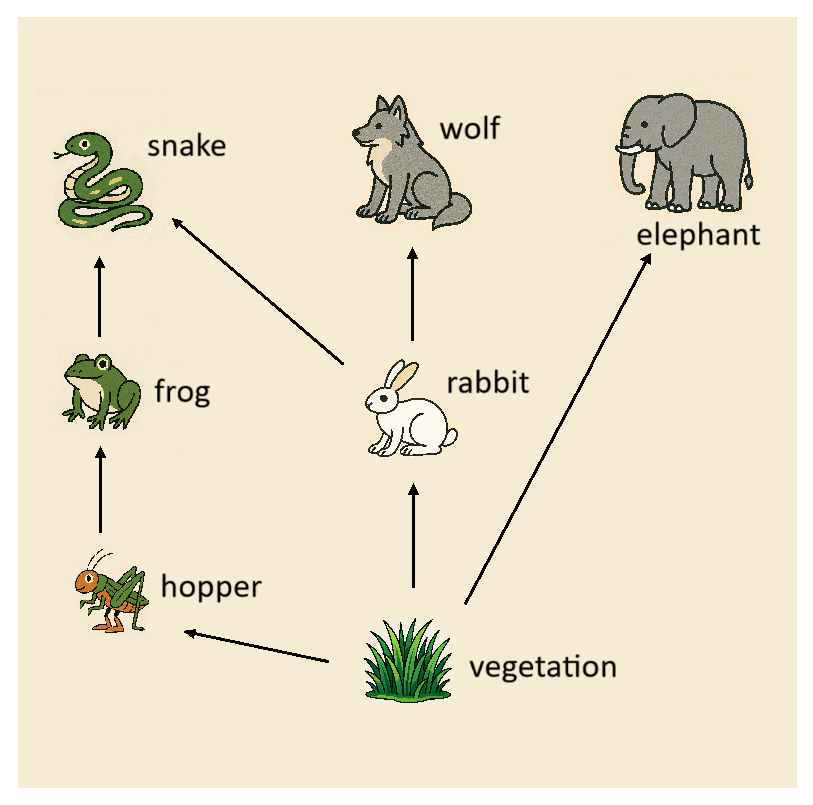
\includegraphics{images/food_web.png}
    }
}
\subfloat[The Food Chain Game\textsuperscript{1}]{
    \resizebox*{0.48\textwidth}{!}{
        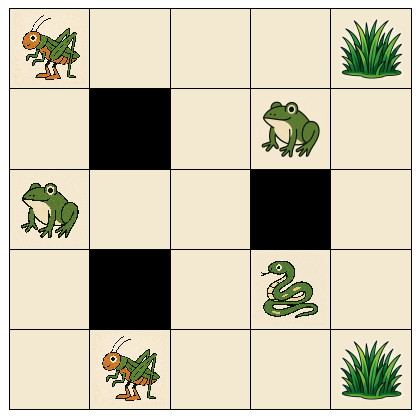
\includegraphics{images/food_chain_game.png}
    }
}
\caption[Caption for LOF]{(a), A food web represents a simple ecosystem. The food web is a cluster of multiple food chains showing what-eats-what. The arrows point in the direction of the energy flow. (b), In the Food Chain game, an agent represents an individual animal of some type. They navigate on a playground trying to feed themselves while avoiding enemies.}
\label{fig:food_chain_game}
\end{figure}
\footnotetext[1]{The individual animal avatars were generated by ChatGPT GPT-4-turbo model which includes image generation via DALL·E 3, provided by OpenAI.}

The game is played on a $w \times h$ grid. Each agent is placed in one of the tiles. There are also obstacles placed on the map. These could be randomly generated using a procedural algorithm or predefined. The state space $S$ contains all possible configurations of the $w \times h$ game board. A game board configuration includes the current timestep $t$, as well as the locations of all the agents, vegetation and obstacles. All positions $(x, y)$ must be unique and satisfy $1 \le x \le w, 1 \le y \le h$. Any state could be an initial state. A state is terminal if $t$ reaches some preset maximum timestep. The action space $A = \{\textbf{up, down, left, right, pass}\}$ is the same for all agents. The state transition function maps the current state and the choices of actions to the next state by executing the agents' actions in a natural way. Agents choose their actions to move along the direction by one cell. Moves resulting in an illegal position will be regarded as pass. If multiple agents try to occupy the same cell, only a randomly selected agent will succeed and the rest will execute the pass action. If an agent is moving away from its current cell, then it is allowed for another agent to enter this cell without conflicts, unless two agents are trying to swap location (this rule prevents agents from passing through each other). The reward function works as follows. After the state transition, if a predator is adjacent to (i.e. within a Manhattan distance of 1) a prey, the prey dies and is removed from the game. Agents receive some negative reward (-1 by default) when they die. Each empty tile also has a chance to grow vegetation each turn. Vegetation is part of the food web and will be destroyed when an agent enter the tile. If the vegetation is a prey to the agent, it will be consumed (this is different from agents eating agents where they only need to be adjacent). Agents get reward (0.1 by default) when they eat. If multiple predators capture a prey at the same time, they must share the reward equally.

The size of the state space grows exponentially with respect to the size of the map and the number of agents. The number of possible states in a game with $n$ agents playing on a board of $k$ cells is lower bounded by $C{k \choose n}$. This computational complexity eliminates any tabular method, a brute-force approach that simply records the value of all possible state-action pairs in a table. Function approximation methods, such as deep neural networks or Monte Carlo methods should be used to solve the whole game \cite{silver2016mastering}. The game is still simple enough to be human playable. The mechanics of the game (the state transition function) is straightforward, so that agents can focus on interactions. Because of the large state space, it is difficult for us to check whether the agents converged to a global NE since it is NP-Hard. However, the way predators hunt for preys often force agents to address the mixed policy problem, as we will explain in the next section with two example scenarios illustrated in Figure~\ref{fig:biased_rps_in_food_chain} and Figure~\ref{fig:tree_maze_chase}. We can actually check whether the agents converge to NEs in those subcases. In summary:
\begin{itemize}
    \item The navigation in the environment where agents are placed is simple enough, so the agents can focus on learning interactions instead of the state transitions, yet the game is still complex enough to be interesting as it blocks out brute-force algorithms.
    \item The game is extendable in many dimensions, the number of agents of each type, the number of species, the relationship between the species, and the size of the map.
    \item The game forces the agents to constantly address the mixed strategy problem.
    \item We can analyse the performance of the agents with game theory.
\end{itemize}

\section{Experimental Evaluation}
Too see how Food Chain can turn on/off the necessary condition (\ref{eq:necessary_condition}) for IVBL to converge, we design two scenarios. The key difference between the two is that one satisfies the condition (\ref{eq:necessary_condition}) and the other does not. We define a simple food web consisting of frogs and hoppers. Hoppers (represented by h) can consume vegetation (drawn as *) and will be eaten by frogs (f). Both scenarios turns off vegetation generation.

\begin{figure}
\centering
    \begin{minipage}{0.48\textwidth}
        \centering
        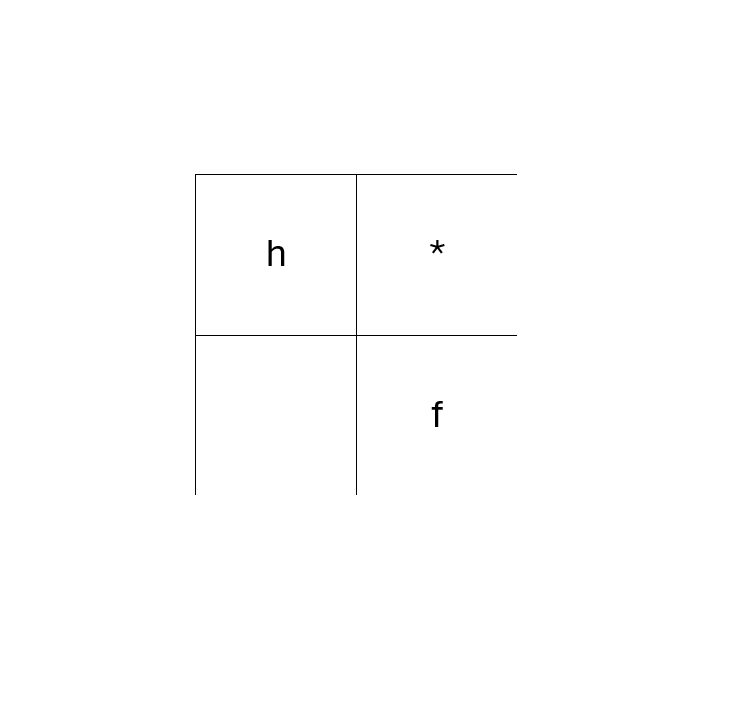
\includegraphics[width=0.931\textwidth]{images/biased_rps.png}
        \caption{The initial state of Biased RPS in Food Chain. The frog (f) is trying to capture the hopper (h). The only NE in the game contains non-uniformly random mixed policies.}
        \label{fig:biased_rps_in_food_chain}
    \end{minipage}\hfill
    \begin{minipage}{0.48\textwidth}
        \centering
        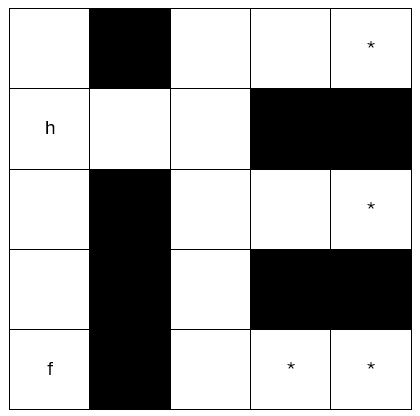
\includegraphics[width=0.9\textwidth]{images/tree_maze_chase.png}
        \caption{The initial state of Tree Maze Chase in Food Chain. The frog (f) is chasing the hopper (h) in the maze. There is an optimal pure (deterministic) policy for both players.}
        \label{fig:tree_maze_chase}
    \end{minipage}
\end{figure}

\subsection{Biased Rock-Paper-Scissors in Food Chain}
This case violates condition (\ref{eq:necessary_condition}). The initial state of the scenario consists of a frog trying to hunt down a hopper as shown in Figure~\ref{fig:biased_rps_in_food_chain}. We can see that in some cases the hopper can escape. If they both pass, they will face the exact same situation again. Figure~\ref{fig:biased_rps_in_food_chain_possible_next_states} in the appendix shows all possible next states. We set the max timestep to 1, so the scenario becomes a normal form game. To break the symmetry so that condition (\ref{eq:necessary_condition}) is violated, we add vegetation in one cell, making the scenario essentially biased RPS. We also raise the feeding reward for both agents to 0.5 to highlight the asymmetry. The reward matrix is shown in Table~\ref{table:biased_rps_in_food_chain_reward_matrix} in the appendix. We can verify that there is a unique NE in the game.
\begin{equation}
    \pi_h=(P(r)=\frac{1}{3},P(d)=\frac{1}{3},P(p)=\frac{1}{3})
    \label{eq:biased_rps_in_food_chain_hopper_policy}
\end{equation}
\begin{equation}
    \pi_f=(P(l)=\frac{1}{13},P(u)=\frac{6}{13},P(p)=\frac{6}{13})
    \label{eq:biased_rps_in_food_chain_frog_policy}
\end{equation}
The expected reward for the hopper and the frog should be $-7/13 \approx -0.538$ and $1/3 \approx 0.333$, respectively.

In the Food Chain game, because all agents have the same mobility, a predator can only capture a prey by trapping them in a corner. Thus, any predator, unless working in a team, has to face this subcase at some point during a general Food Chain game played on an open ground. The scenario represents a subgame which shows up frequently in a full game.

\subsection{Tree Maze Chase in Food Chain}
This scenario essentially turns off the mixed policy problem. We set up the initial state as shown in Figure~\ref{fig:tree_maze_chase} where a frog is chasing a hopper in a maze. This map resembles a tree structure (no cycles) which creates a pure NE, because there is always an optimal action. The hopper should go for the tunnel with more vegetation and the frog should simply chase the hopper. The necessary condition (\ref{eq:necessary_condition}) is satisfied. To make sure that at most two vegetations can be picked up by the hopper, we set the max timestep to 12. The optimal rewards for the hopper and the frog are -0.8 and 1, respectively.

\subsection{Results and Discussion}
We tested the IVBL algorithm IQL and the independent policy-based algorithm IPPO in both scenarios. The experiments were run using the open-source MARL library BenchMARL \cite{bettini2024benchmarl}. All experiments ran for 800 iterations. For each iteration, the algorithm collects 640 timesteps as training samples and train the neural network before 50 evaluation games were run. The plots show the average reward for each agent during the evaluation phase. Each experiment was run 20 times to mitigate the effect of randomness and the graphs show the boots trapped 95\% confidence interval. More details of the parameters for the experiments can be found in Table~\ref{table:experiments_parameters} in the appendix.

\begin{figure}
\centering
\subfloat[Biased RPS Hopper Rewards]{
    \resizebox*{0.48\textwidth}{!}{
        \includesvg{plots/food_chain_biased_rps_hopper_return.svg}
    }
}
\subfloat[Biased RPS Frog Rewards]{
    \resizebox*{0.48\textwidth}{!}{
        \includesvg{plots/food_chain_biased_rps_frog_return.svg}
    }
}
\caption{Biased RPS. IVBL (IQL) shows significantly more instability and does not converge to the NE.}
\label{fig:biased_rps_in_food_chain_rewards}
\end{figure}

\begin{figure}
\centering
\subfloat[Tree Maze Chase Hopper Rewards]{
    \resizebox*{0.48\textwidth}{!}{
        \includesvg{plots/food_chain_tree_maze_chase_hopper_return.svg}
    }
}
\subfloat[Tree Maze Chase Frog Rewards]{
    \resizebox*{0.48\textwidth}{!}{
        \includesvg{plots/food_chain_tree_maze_chase_frog_return.svg}
    }
}
\caption{Tree Maze Chase. Both algorithms quickly learned to play the game and tend to stay in the optimal reward range. Note that increasing frog reward reduces the hopper reward as the game is non-cooperative.}
\label{fig:tree_maze_chase_rewards}
\end{figure}

Figure~\ref{fig:biased_rps_in_food_chain_rewards} demonstrates the performance of the algorithms in the biased RPS scenario where the necessary condition (\ref{eq:necessary_condition}) for IVBL to converge is not met. The results show that the IVBL algorithm IQL failed to converge to a defined solution range and were struggling to stabilize itself. The hopper's reward fluctuates between -1 and -0.2, where the optimal value is -0.538. These value can be as far as 85\% away from the desired amount. The frog reward oscillates in the range [0.2, 0.5], which is in a $\pm 70\%$  range from the actual NE (0.333). For comparison, the independent policy-based learning algorithm IPPO achieves a reward that stays more in the optimal range and is far more stable which indicates the agents are converging towards the NE.

In contrast, IVBL does significantly better in the tree maze scenario, as shown in Figure~\ref{fig:tree_maze_chase_rewards}. This time, the game scenario satisfies the condition (\ref{eq:necessary_condition}). Although still unstable, IQL can roughly reach the optimal reward at the end. The optimal rewards for the hopper and the frog are -0.8 and 0.1, respectively. Even in this case, the policy-based method still appears to be more reliable than IVBL.

\section{Conclusion}
In this work, we have analysed the stability of independent value-based learning (IBVL) algorithms in non-cooperative games and tested their performance in specific game scenarios. By means of proof by contradiction and the design of experiments based on the proposed Food Chain game, we found that the studied algorithms only converge to Nash equilibrium (NE) in non-cooperative settings when every agent's policy evenly chooses the next action among their worthy actions (actions that are played with a positive probability). This explains why promising results are achieved when applying IVBL to games with pure NE, including cooperative games.

This work also proposes the Food Chain game which has certain traits ---such as ease of navigation, focus on interactions, and extendability, among others--- that are instrumental for the analysis of the stability in non-cooperative settings. The test results show that IVBL algorithms perform poorly in scenarios where the identified condition is violated. Our work is limited to small two-player scenarios in the Food Chain game. There are still interesting characteristics of the game that will be explored in the future. Such as the extension in both the number of agents and the number of species on the food web.

\section*{Funding}
This research was funded by the University of the West of England.

\bibliographystyle{tfnlm}
\bibliography{ref}

\pagebreak
\appendix

\section{Biased RPS in Food Chain}
Figure~\ref{fig:biased_rps_in_food_chain_possible_next_states} shows all the possible next state of the Biased RPS scenario in Food Chain. Table~\ref{table:biased_rps_in_food_chain_reward_matrix} describes the reward matrix of the scenario (note that if both agents try to move into the vegetation tile, the hopper only has a 50\% chance to get the vegetation).

\begin{figure}
\centering
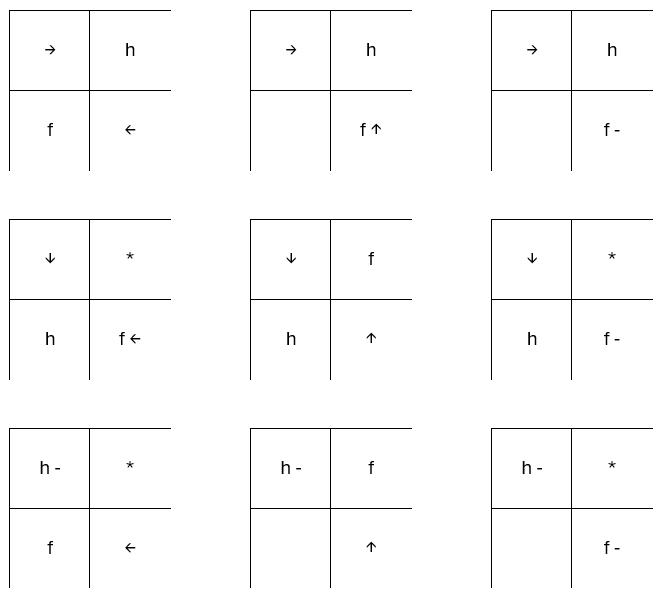
\includegraphics{images/biased_rps_possible_next_states.png}
\caption{Possible Next States in Biased RPS in Food Chain (omitting illegal moves)}
\label{fig:biased_rps_in_food_chain_possible_next_states}
\end{figure}

\begin{table}
\tbl{Biased RPS in Food Chain Reward Matrix}{
    \begin{tabular}{l|ccc}
        & left & up & pass\\
        \hline
        right & 0.5,0 & -0.75,0.5 & -0.5,0.5 \\
        down & -1,0.5 & 0,0 & -1,0.5 \\
        pass & -1,0.5 & -1,0.5 & 0,0 \\
    \end{tabular}
}
\tabnote{Hopper is the row player.}
\label{table:biased_rps_in_food_chain_reward_matrix}
\end{table}

\section{Experiments Parameters}
\begin{table}
\tbl{Experiments Parameters}{
    \begin{tabular}{lcc}
        \toprule
        \multicolumn{3}{l}{game parameters} \\
        \midrule
        & Biased RPS & Tree Maze Chase \\
        \cmidrule{2-3}
        size of the map & $2 \times 2$ & $5 \times 5$ \\
        max timestep & 1 & 12 \\
        feeding reward & 0.5 & 0.1 \\
        death reward & \multicolumn{2}{c}{-1} \\
        vegetation spawn chance & \multicolumn{2}{c}{0} \\
        number of agents & \multicolumn{2}{c}{2} \\
        agent types & \multicolumn{2}{c}{2} \\
        \midrule
        \multicolumn{3}{l}{experiment parameters} \\
        \midrule
        repetitions of each experiment & \multicolumn{2}{c}{20} \\
        number of iterations & \multicolumn{2}{c}{800} \\
        evaluation games after each iteration & \multicolumn{2}{c}{50} \\
        \midrule
        \multicolumn{3}{l}{training hyper parameters} \\
        \midrule
        & IPPO & IQL \\
        \cmidrule{2-3}
        on-policy minibatch optimization iterations\textsuperscript{a} & 10 & \\
        off-policy optimizer steps\textsuperscript{b} & & 100 \\
        off-policy memory buffer size & & 20,000 \\
        frames collected for each iteration & \multicolumn{2}{c}{640} \\
        minibatch size & \multicolumn{2}{c}{32} \\
        discount factor $\gamma$ & \multicolumn{2}{c}{0.99} \\
        learning rate $\alpha$ & \multicolumn{2}{c}{$5 \times 10^{-5}$} \\
        the $\varepsilon$ parameter of the adam optimizer & \multicolumn{2}{c}{$1 \times 10^{-6}$} \\
        \bottomrule
    \end{tabular}
}
\tabnote{\textsuperscript{a}The number of times collected frames will be split into minibatches and trained. \\ \textsuperscript{b}The number of times a minibatch will be sampled from the memory buffer and trained over.}
\label{table:experiments_parameters}
\end{table}

\end{document}